\documentclass[12pt]{article}
\usepackage{amsmath}
\usepackage{graphicx}
\usepackage{hyperref}
\usepackage{listings}
\usepackage{color}
\usepackage{pythonhighlight}
\usepackage{xcolor}

\title{Operating System Course Report - First Half of the Semester}
\author{A class}
\date{\today}

\begin{document}

\maketitle
\newpage

\tableofcontents
\newpage

\section{Introduction}
This report summarizes the topics covered during the first half of the Operating System course. It includes theoretical concepts, practical implementations, and assignments. The course focuses on the fundamentals of operating systems, including system architecture, process management, CPU scheduling, and deadlock handling.

\section{Course Overview}
\subsection{Objectives}
The main objectives of this course are:
\begin{itemize}
    \item To understand the basic components and architecture of a computer system.
    \item To learn process management, scheduling, and inter-process communication.
    \item To explore file systems, input/output management, and virtualization.
    \item To study the prevention and handling of deadlocks in operating systems.
\end{itemize}

\subsection{Course Structure}
The course is divided into two halves. This report focuses on the first half, which covers:
\begin{itemize}
    \item Basic Concepts and Components of Computer Systems
    \item System Performance and Metrics
    \item System Architecture of Computer Systems
    \item Process Description and Control
    \item Scheduling Algorithms
    \item Process Creation and Termination
    \item Introduction to Threads
    \item File Systems
    \item Input and Output Management
    \item Deadlock Introduction and Prevention
    \item User Interface Management
    \item Virtualization in Operating Systems
\end{itemize}

\section{Topics Covered}

\subsection{Basic Concepts and Components of Computer Systems}
This section explains the fundamental components that make up a computer system, including the CPU, memory, storage, and input/output devices.

\subsection{System Performance and Metrics}
This section introduces various system performance metrics used to measure the efficiency of a computer system, including throughput, response time, and utilization.

\subsection{System Architecture of Computer Systems}
Describes the architecture of modern computer systems, focusing on the interaction between hardware and the operating system.

\subsection{Process Description and Control}
Processes are a central concept in operating systems. This section covers:
\begin{itemize}
    \item Process states and state transitions
    \item Process control block (PCB)
    \item Context switching
\end{itemize}

\subsection{Scheduling Algorithms}
This section covers:
\begin{itemize}
    \item First-Come, First-Served (FCFS)
    \item Shortest Job Next (SJN)
    \item Round Robin (RR)
\end{itemize}
It explains how these algorithms are used to allocate CPU time to processes.

\subsection{Process Creation and Termination}
Details how processes are created and terminated by the operating system, including:
\begin{itemize}
    \item Process spawning
    \item Process termination conditions
\end{itemize}

\subsection{Introduction to Threads}
This section introduces the concept of threads and their relation to processes, covering:
\begin{itemize}
    \item Single-threaded vs. multi-threaded processes
    \item Benefits of multithreading
\end{itemize}

\begin{figure}[h]
    \centering
    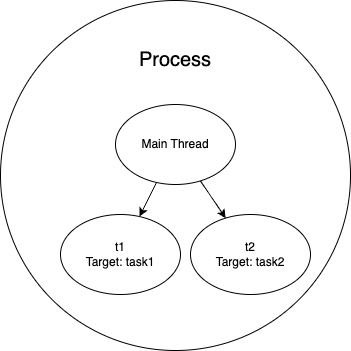
\includegraphics[width=0.5\textwidth]{/Users/khawaritzmi/Unhas/os_report_mid2024/a_class/asset/example.png}  % Sesuaikan nama file dan ukurannya
    \caption{Ini adalah gambar contoh dari multithreading.}
    \label{fig:contoh_gambar}
\end{figure}

Seperti yang terlihat pada Gambar \ref{fig:contoh_gambar}, inilah cara menambahkan gambar dengan keterangan.

\subsection{File Systems}
File systems provide a way for the operating system to store, retrieve, and manage data. This section explains:
\begin{itemize}
    \item File system structure
    \item File access methods
    \item Directory management
\end{itemize}

\subsection{Input and Output Management}
Input and output management is key for handling the interaction between the system and external devices. This section includes:
\begin{itemize}
    \item Device drivers
    \item I/O scheduling
\end{itemize}

\subsection{Deadlock Introduction and Prevention}
Explores the concept of deadlocks and methods for preventing them:
\begin{itemize}
    \subsubsection{Pengenalan \textit{Deadlock}}
        \begin{enumerate}
            \item \textbf{Pengertian \textit{Deadlock}}
            \item \textbf{Kondisi Terjadinya \textit{Deadlock}}
            \item \textbf{Model \textit{Deadlock}}

                \hspace{1cm}
                Model \textit{deadlock} adalah representasi dari situasi dimana serangkaian proses dalam suatu sistem tidak dapat melanjutkan eksekusi karena saling menunggu sumber daya yang sedang digunakan oleh proses lain.\newline
                
                \begin{enumerate}
                    \item \textit{\textbf{Resource Alocation Graph}}

                        \hspace{1cm}
                        Sebuah model graf yang digunakan untuk mempresentasikan hubungan antara proses dan sumber daya dalam sistem komputasi.

                        \hspace{1cm}
                        Menurut Wahid (2020), untuk menggambar model 
                        
                        \textit{resource allocation graph} ada beberapa ketentuan sebagai berikut:
                        
                        \begin{itemize}
                            \item \textbf{Persegi} menandakan sebuah sumber daya atau \textit{resource} yang biasa diberi penanda "R(n)", jumlah \textit{resource} yang bisa digunakan biasa ditandai dengan jumlah titik yang ada dalam persegi tersebut.
                            
                            \item \textbf{Lingkaran} menandakan sebuah proses dengan penanda huruf "P(n)".
                            
                            \item \textbf{Lingkaran} $\longrightarrow$ \textbf{Persegi} menandakan bahwa proses tersebut sedang meminta sebuah sumber daya dari \textit{resource}. 
                            
                            \item \textbf{Persegi} $\longrightarrow$ \textbf{Lingkaran} menandakan bahwa sumber daya dari \textit{resource} sedang digunakan oleh proses tersebut.\newline
                        \end{itemize}

                        \begin{figure}[h]
                            \centering
                            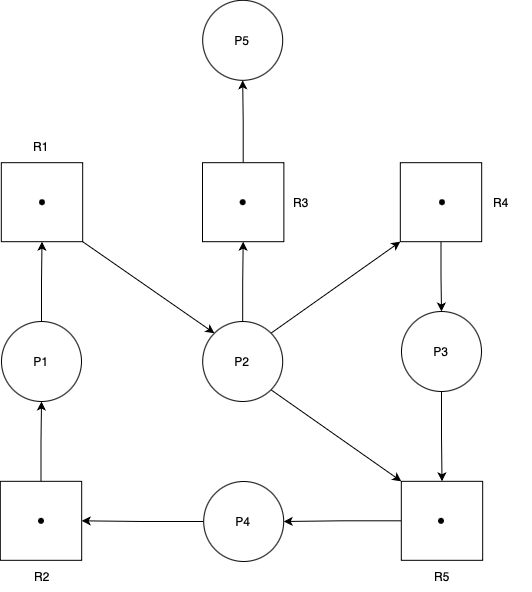
\includegraphics[width=0.45\linewidth]
                            {asset/RAG.drawio.png}
                            \caption{Contoh Diagram \textit{Deadlock} dalam RAG}
                            \label{fig:deadlock-RAG}
                            \end{figure}
                        
                    \item \textit{\textbf{State-based Model}}

                        \hspace{1cm}
                        Model yang digunakan untuk menganalisa dan mendeteksi \textit{deadlock} dengan melihat keadaan (\textit{state}) sistem dalam hal alokasi sumber daya dan proses yang sedang berjalan.

                        \hspace{1cm}
                        Gambar dibawah adalah contoh ilustrasi dari \textit{state-based model} yang biasa digunakan untuk menentukan apakah sistem berada dalam kondisi \textit{safe} atau \textit{unsafe}. Sistem bisa dikatakan dalam \textit{state} aman jika sistem dapat mengalokasikan sumber daya untuk setiap proses secara berurutan dan menghindari \textit{deadlock}.
                        
                        \hspace{1cm}
                        Untuk menentukan apakah sistem berada dalam kondisi \textit{safe} atau \textit{unsafe} kita bisa menggunakan \textit{safety algorithm} atau \textit{banker algorithm}.\newline

                        \begin{figure}[h]
                            \centering
                            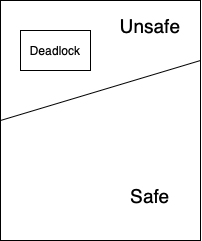
\includegraphics[width=0.45\linewidth]
                            {asset/WFG.drawio.png}
                                \caption{Contoh Model \textit{State-based} model}
                            \label{fig:deadlock-SBM}
                            \end{figure}
                        
                    \item \textit{\textbf{Wait-for Graph}}

                        \hspace{1cm}
                        Model ini adalah penyederhanaan dari \textit{resource allocation graph}. Dalam \textit{wait-for graph} hanya proses yang diwakili sebagai \textit{node}, dan ada panah yang menunjukkan bahwa satu proses menunggu proses lain untuk melepaskan sumber daya.
                            \begin{figure}[h]
                            \centering
                            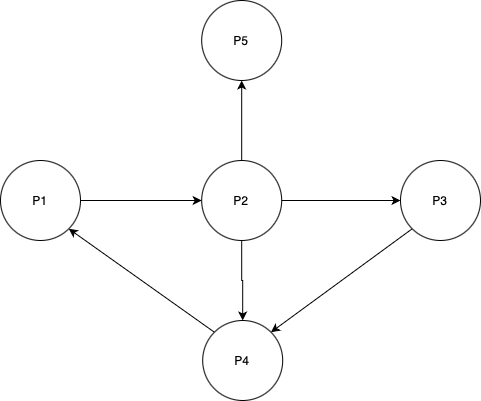
\includegraphics[width=0.4\linewidth]
                            {asset/WFG1.drawio.png}
                            \caption{Contoh Diagram Deadlock dalam WFG}
                            \label{fig:deadlock-WFG}
                            \end{figure}

                        \hspace{1cm}
                        Model \textit{wait-for graph} biasa digunakan untuk menyederhanakan hasil dari model \textit{resource allocation graph}, tapi ada beberapa syarat yang harus terpenuhi jika ingin mengubah \textit{resource allocation graph} menjadi model \textit{wait-for graph}, adapun syarat dan ketentuannya sebagai berikut : 
                        \begin{itemize}
                            \item Tidak ada \textit{resource}, jadi model \textit{wait-for graph} hanya dapat menampilkan proses tanpa menampilkan \textit{resource}.
                            
                            \item  Mengubah relasi proses-\textit{resource} menjadi antar proses.\newline
                        \end{itemize}

                \end{enumerate}
            \item \textbf{Deteksi dan Pemulihan \textit{Deadlock}}
        \end{enumerate}
    \subsubsection{ \textit{Deadlock prevention techniques}}
\end{itemize}

\subsection{User Interface Management}
This section discusses the role of the operating system in managing the user interface. Topics covered include:
\begin{itemize}
    \item Graphical User Interface (GUI)
    \item Command-Line Interface (CLI)
    \item Interaction between the user and the operating system
\end{itemize}

\subsection{Virtualization in Operating Systems}
Virtualization allows multiple operating systems to run concurrently on a single physical machine. This section explores:
\begin{itemize}
    \item Concept of virtualization
    \item Hypervisors and their types
    \item Benefits of virtualization in modern computing
\end{itemize}

\section{Assignments and Practical Work}
\subsection{Assignment 1: Process Scheduling}
Students were tasked with implementing various process scheduling algorithms (e.g., FCFS, SJN, and RR) and comparing their performance under different conditions.
\subsubsection{Group 1}
\begin{python}
    class Process:
    def __init__(self, pid, arrival_time, burst_time):
        self.pid = pid
        self.arrival_time = arrival_time
        self.burst_time = burst_time
        self.completion_time = 0
        self.turnaround_time = 0
        self.waiting_time = 0
\end{python}

\begin{table}[htbp] % Optional: For floating position
    \centering
    \begin{tabular}{|c|c|c|} % Defines number of columns and alignment (c = center, l = left, r = right). '|' creates vertical lines.
    \hline
    Header 1 & Header 2 & Header 3 \\ % Column headers
    \hline
    Row 1, Column 1 & Row 1, Column 2 & Row 1, Column 3 \\ % First row of data
    \hline
    Row 2, Column 1 & Row 2, Column 2 & Row 2, Column 3 \\ % Second row of data
    \hline
    \end{tabular}
    \caption{Your table caption} % Optional: For adding a caption
    \label{tab:your_label} % Optional: For cross-referencing the table
\end{table}
\subsection{Assignment 2: Deadlock Handling}
In this assignment, students were asked to simulate different deadlock scenarios and explore various prevention methods.

\subsection{Assignment 3: Multithreading and Amdahl's Law}
This assignment involved designing a multithreading scenario to solve a computationally intensive problem. Students then applied **Amdahl's Law** to calculate the theoretical speedup of the program as the number of threads increased.

\subsubsection{Group 10}
\begin{enumerate}
    \item Sebuah program memiliki 75\% bagian yang dapat diparalelkan. Jika program ini dijalankan pada sistem dengan enam \textit{core} prosesor, berapakah \textit{speedup} maksimum yang dapat dicapai menurut Hukum Amdahl?

    \textbf{Jawaban : }
    \begin{python}
    import math

    def calculate_speedup(parallel_fraction, num_processors):
        serial_fraction = 1 - parallel_fraction
        return 1 / (serial_fraction + (parallel_fraction / num_processors))
    
    # Problem parameters
    parallel_percentage = 75  # 75% can be parallelized
    num_cores = 6
    
    # Convert percentage to fraction
    parallel_fraction = parallel_percentage / 100
    
    # Calculate speedup
    speedup = calculate_speedup(parallel_fraction, num_cores)
    
    print(f"Untuk program dengan {parallel_percentage}% kode yang dapat diparalelkan berjalan pada {num_cores} cores:")
    print(f"Kecepatan maksimum menurut Amdahl's Law adalah: {speedup:.2f}x")
    
    # Calculate theoretical maximum speedup (with infinite cores)
    max_theoretical_speedup = calculate_speedup(parallel_fraction, math.inf)
    print(f"Kecepatan maksimum teoritis (dengan cores tak terbatas) adalah: {max_theoretical_speedup:.2f}x")
\end{python}

    \textbf{Penjelasan : }
    \begin{enumerate}
        \item Kita mengimpor modul \textit{math} untuk menggunakan konstanta \textit{inf} (tak terhingga) nanti.
        
        \item Membuat fungsi \textit{calculate\_speedup} yang menerima dua parameter:
            \begin{itemize}
                \item \textit{parallel\_fraction}: Bagian program yang dapat diparalelkan (0-1).
                
                \item \textit{num\_processors}: Jumlah prosesor atau \textit{thread} yang digunakan.
            \end{itemize}
            
        \item Implementasi Hukum Amdahl:
            \begin{itemize}
                \item Ini adalah implementasi langsung dari rumus Hukum Amdahl: \textit{Speedup} = 1 / ((1 - P) + (P / N)).
                
                \item \textit{serial\_fraction} adalah bagian yang tidak dapat diparalelkan (1 - P).
                
                \item Rumus menghitung \textit{speedup} berdasarkan fraksi paralel dan jumlah prosesor.
            \end{itemize}
            
        \item Pengaturan parameter masalah :
            \begin{itemize}
                \item Sesuai soal, 75\% program dapat diparalelkan dan menggunakan enam \textit{core}.
            \end{itemize}
            
        \item Konversi persentase ke fraksi :
            \begin{itemize}
                \item Mengubah 75\% menjadi 0.75 untuk perhitungan.
            \end{itemize}
            
        \item Perhitungan \textit{speedup} :
            \begin{itemize}
                \item Memanggil fungsi dengan parameter yang telah ditentukan.
            \end{itemize}
            
        \item  Mencetak hasil :
            \begin{itemize}
                \item Menampilkan hasil perhitungan dengan format yang mudah dibaca.
                \item .2f memformat angka dengan dua desimal.
            \end{itemize}
            
        \item  Perhitungan \textit{speedup} teoritis maksimum :
            \begin{itemize}
                \item Menghitung \textit{speedup} dengan jumlah prosesor tak terbatas (\textit{math.inf}).
                
                \item Ini menunjukkan batas atas teoritis dari \textit{speedup} yang mungkin dicapai.
            \end{itemize}
            
        \item Mencetak \textit{speedup} teoritis maksimum :
            \begin{itemize}
                \item Menampilkan batas atas teoritis \textit{speedup}.
            \end{itemize}
            
    \end{enumerate}
\end{enumerate}

\subsection{Assignment 4: Simple Command-Line Interface (CLI) for User Interface Management}
Students were tasked with creating a simple **CLI** for user interface management. The CLI should support basic commands such as file manipulation (creating, listing, and deleting files), process management, and system status reporting.

\subsubsection{Group 10}
\begin{enumerate}
    \item Buatlah sebuah \textit{Command Line Interface} (CLI) sederhana untuk manajemen antarmuka pengguna. CLI harus mendukung perintah dasar seperti manipulasi \textit{file} (membuat, membuat daftar, dan menghapus \textit{file}), manajemen proses, dan status sistem pelaporan.

    \textbf{Jawaban :}
    \begin{python}
        import os
import psutil
import sys

def create_file(filename):
    try:
        with open(filename, 'w') as f:
            pass
        print(f"File '{filename}' berhasil dibuat.")
    except IOError:
        print(f"Gagal membuat file '{filename}'.")

def list_files():
    files = os.listdir()
    for file in files:
        print(file)

def delete_file(filename):
    try:
        os.remove(filename)
        print(f"File '{filename}' berhasil dihapus.")
    except FileNotFoundError:
        print(f"File '{filename}' tidak ditemukan.")
    except PermissionError:
        print(f"Tidak memiliki izin untuk menghapus file '{filename}'.")

def list_processes():
    for proc in psutil.process_iter(['pid', 'name']):
        print(f"PID: {proc.info['pid']}, Name: {proc.info['name']}")

def system_status():
    print(f"CPU Usage: {psutil.cpu_percent()}%")
    print(f"Memory Usage: {psutil.virtual_memory().percent}%")
    print(f"Disk Usage: {psutil.disk_usage('/').percent}%")

def main():
    while True:
        print("\nSimple CLI Manager")
        print("1. Buat File")
        print("2. Daftar File")
        print("3. Hapus File")
        print("4. Daftar Proses")
        print("5. Status Sistem")
        print("6. Keluar")
        
        choice = input("Pilih opsi (1-6): ")
        
        if choice == '1':
            filename = input("Masukkan nama file: ")
            create_file(filename)
        elif choice == '2':
            list_files()
        elif choice == '3':
            filename = input("Masukkan nama file yang akan dihapus: ")
            delete_file(filename)
        elif choice == '4':
            list_processes()
        elif choice == '5':
            system_status()
        elif choice == '6':
            print("Terima kasih telah menggunakan Simple CLI Manager.")
            sys.exit()
        else:
            print("Pilihan tidak valid. Silakan coba lagi.")

if __name__ == "__main__":
    main()
    \end{python}
    
    \textbf{Penjelasan :}
    \begin{enumerate}
        \item Kita mengimpor modul-modul yang diperlukan:
            \begin{itemize}
                \item \textit{os} untuk operasi \textit{file} dan sistem.
                
                \item \textit{psutil} untuk manajemen proses dan pemantauan status sistem.
                
                \item \textit{sys} untuk fungsi-fungsi terkait sistem, termasuk keluar dari program.
            \end{itemize}
            
        \item Fungsi utama :
            \begin{itemize}
                \item \textit{create\_file(filename)}: Membuat \textit{file} baru.
                
                \item \textit{list\_files()}: Menampilkan daftar \textit{file} di direktori saat ini.
                
                \item \textit{delete\_file(filename)}: Menghapus \textit{file} yang ditentukan.
                
                \item \textit{list\_processes()}: Menampilkan daftar proses yang sedang berjalan.
                
                \item \textit{system\_status()}: Menampilkan penggunaan CPU, memori, dan \textit{disk}.
            \end{itemize}
            
        \item Fungsi \textit{main()}:
            \begin{itemize}
                \item Menampilkan menu utama dalam \textit{loop}.
                \item Meminta input dari pengguna.
                \item Memanggil fungsi yang sesuai berdasarkan pilihan pengguna.
            \end{itemize}
            
        \item Kita menggunakan \textit{if \_\_name\_\_ == "\_\_main\_\_"}: 
            \begin{itemize}
                \item untuk memastikan bahwa \textit{main()} hanya dijalankan jika \textit{script} dieksekusi langsung, bukan diimpor sebagai modul.
            \end{itemize}
    \end{enumerate}
\end{enumerate}


\subsection{Assignment 5: File System Access}
In this assignment, students implemented file system access routines, including:
\begin{itemize}
    \item File creation and deletion
    \item Reading from and writing to files
    \item Navigating directories and managing file permissions
\end{itemize}

\section{Conclusion}
The first half of the course introduced core operating system concepts, including process management, scheduling, multithreading, and file system access. These topics provided a foundation for more advanced topics to be covered in the second half of the course.

\begin{thebibliography}{9}
    \bibitem{RAG_GeeksforGeeks}
    GeeksforGeeks. (n.d.). \textit{Resource Allocation Graph (RAG) in operating system}. Retrieved September 20, 2024, from \url{https://www.geeksforgeeks.org/resource-allocation-graph-rag-in-operating-system/}

    \bibitem{DeadlockConditions_GeeksforGeeks}
    GeeksforGeeks. (n.d.).\textit{Conditions for Deadlock in operating system}. Retrieved September 20, 2024, from \url{https://www-geeksforgeeks-org.translate.goog/conditions-for-deadlock-in-operating-system/?_x_tr_sl=en&_x_tr_tl=id&_x_tr_hl=id&_x_tr_pto=tc}

    \bibitem{WaitForGraph_GeeksforGeeks}
    GeeksforGeeks. (n.d.). Wait-for-Graph deadlock detection in distributed system. Retrieved September 20, 2024, from \url{https://www.geeksforgeeks.org/wait-for-graph-deadlock-detection-in-distributed-system/}

    \bibitem{}
    Shoebridge, T. (2023, September 21). What is Deadlock? [Video]. YouTube. Retrieved September 25, 2024, from url{https://youtu.be/VC3UUXCz2UM}

    
\end{thebibliography}

    
\end{document}